\graphicspath{{./assets/}}
\setcounter{mtc}{5}
\chapter{3rd Sprint: Resource provisioning  }
\fancyhead[R]{\ungaramond\small\textbf{Chapter V.  3rd Sprint: Resource provisioning  }}

\minitoc
\newpage
\section*{Introduction}

\section{Sprint Backlog}

\begin{longtable}[H]{|m{1.5cm}|m{3cm}|m{1.5cm}|m{8cm}|}
\hline
{\textbf{Epic ID}} & {\textbf{Epic}} & {\textbf{Story ID}} & {\textbf{Story}}\\
\hline
1  & \raggedright Provisioning resources using IaC playbooks and HCP config files.  &  1.1	 & Preparing provider specific(ovh) terraform config. \\
\cline{3-4}
& & 1.2 & Preparing ansible playbook to initiate provisioning. \\
\cline{3-4}
& & 1.3	& Setting up IaC host machine.  \\
\cline{3-4}
& & 1.4	& Cloud provider account and project creation.  \\
\hline
\caption{3rd Sprint Backlog}
\end{longtable}

% \begin{longtable}[H]{|m{1.5cm}|m{3cm}|m{1.5cm}|m{8cm}|}
% \hline
% \multicolumn{1}{|c|}{\textbf{Epic ID}} & \multicolumn{1}{|c|}{\textbf{Epic}} & \multicolumn{1}{|c|}{\textbf{Story ID}} & \multicolumn{1}{|c|}{\textbf{Story}}\\
% \hline
% \endfirsthead
% \endhead
% \multirow{4}{*}{\textbf{1}}  & \multirow{4}{*}{Provisioning resources using IaC playbooks and HCP config files.} & 1.1 & \begin{tabular}[c]{@{}l@{}}Preparing provider specific(ovh) terraform config. \end{tabular} \\
% \cline{3-4}
% & & 1.2 & \begin{tabular}[c]{@{}l@{}}Preparing ansible playbook to initiate provisioning.\end{tabular}  \\
% \cline{3-4}
% & & \begin{tabular}[c]{@{}l@{}}1.3	\end{tabular} & \begin{tabular}[c]{@{}l@{}}Setting up IaC host machine. \end{tabular}  \\
% \cline{3-4}
% & & \begin{tabular}[c]{@{}l@{}}1.4\end{tabular} 	& \begin{tabular}[c]{@{}l@{}}Cloud provider account and project creation. \end{tabular}  \\
% \hline
% \caption{Table 3rd Sprint Backlog}
% \end{longtable}

\section{UML design : class diagram for cloud infrastructure }
The following diagram showcases the interaction between the infrastructure as code tools and the cloud provider as well as the resulting infrastructure, its components, and the relation between them. 
\begin{figure}[H]\centering
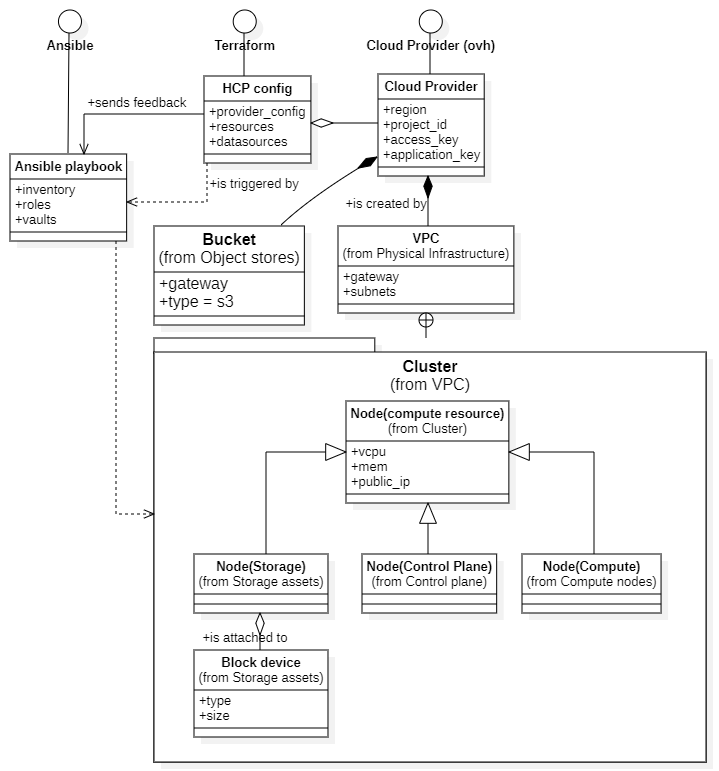
\includegraphics[width=1.0\textwidth,angle=00]{assets/f13.png}
\caption{Class Diagram for cloud infrastructure}
\label{fig:fig13}
\end{figure}

\section{“HCP config” diagram for cloud provisioning: }
The following figure illustrates the main resources declared in our terraform “HCP config”: 

\begin{figure}[H]\centering
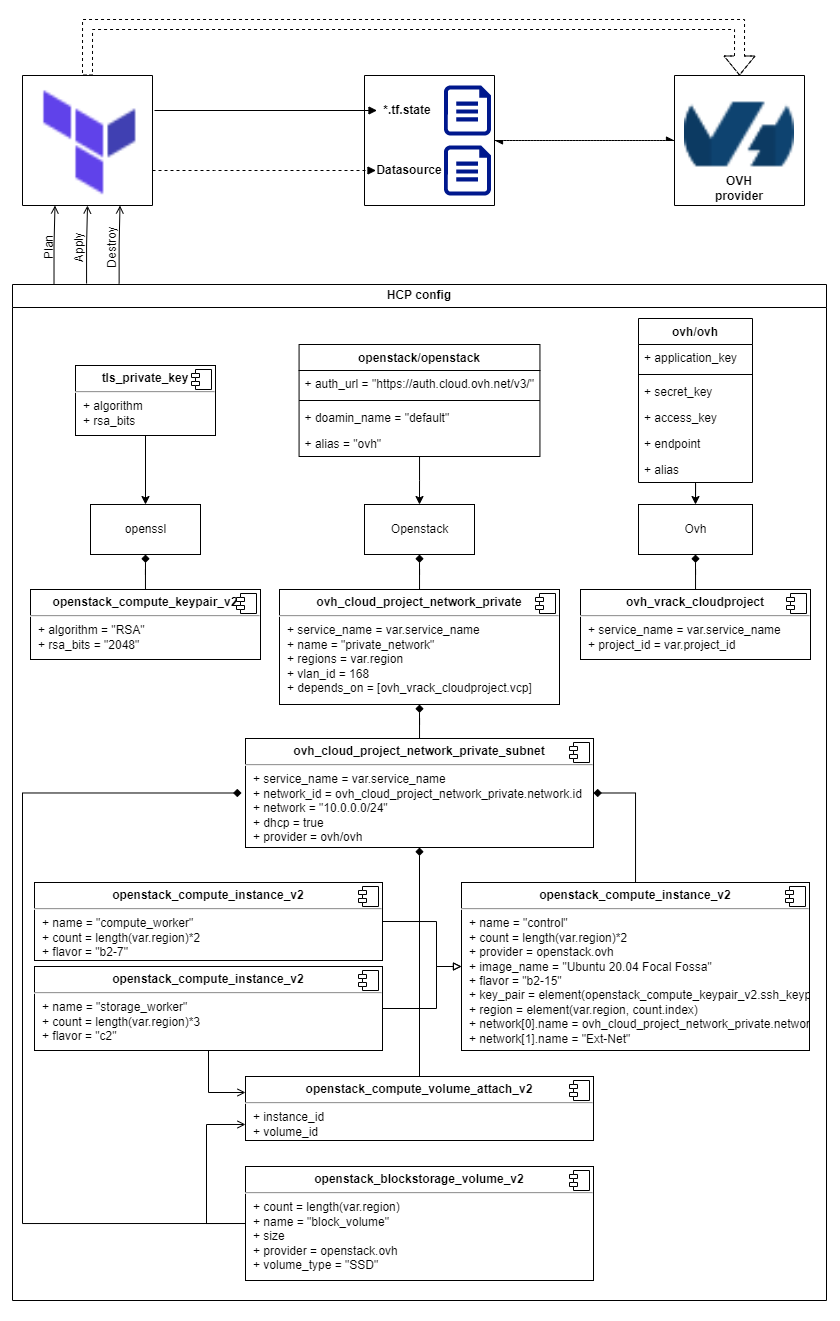
\includegraphics[width=0.95\textwidth]{assets/f14.png}
\caption{Diagram for cloud provisionning}
\label{fig:fig14}
\end{figure}

The diagram shows a Terraform configuration for deploying resources on OVH cloud provider. The configuration consists of four main components: provider, network, compute, and storage. 

\begin{itemize}[label={--}]
\item The provider component specifies the OVH cloud provider and the authentication credentials to access the account. 
\item The network component defines the virtual private cloud (VPC) and its associated resources, such as subnets, security groups, and routers. 
\item The compute component defines the public cloud compute instances that will host our PaaS. The VMs are launched in the subnets defined in the network component, and their configurations are specified through variables. 
\item The storage component defines the object storage bucket that will store application and backup data, and the block storage volumes that will be attached to the VMs. 
\end{itemize}

All the resources are managed by Terraform, which allows for easy provisioning, scaling, and management of the infrastructure. 

Overall, this Terraform configuration with OVH cloud provider provides a scalable, secure, and highly available infrastructure for running applications. 

\section{Component diagram of provisioned resources}

\begin{figure}[H]\centering
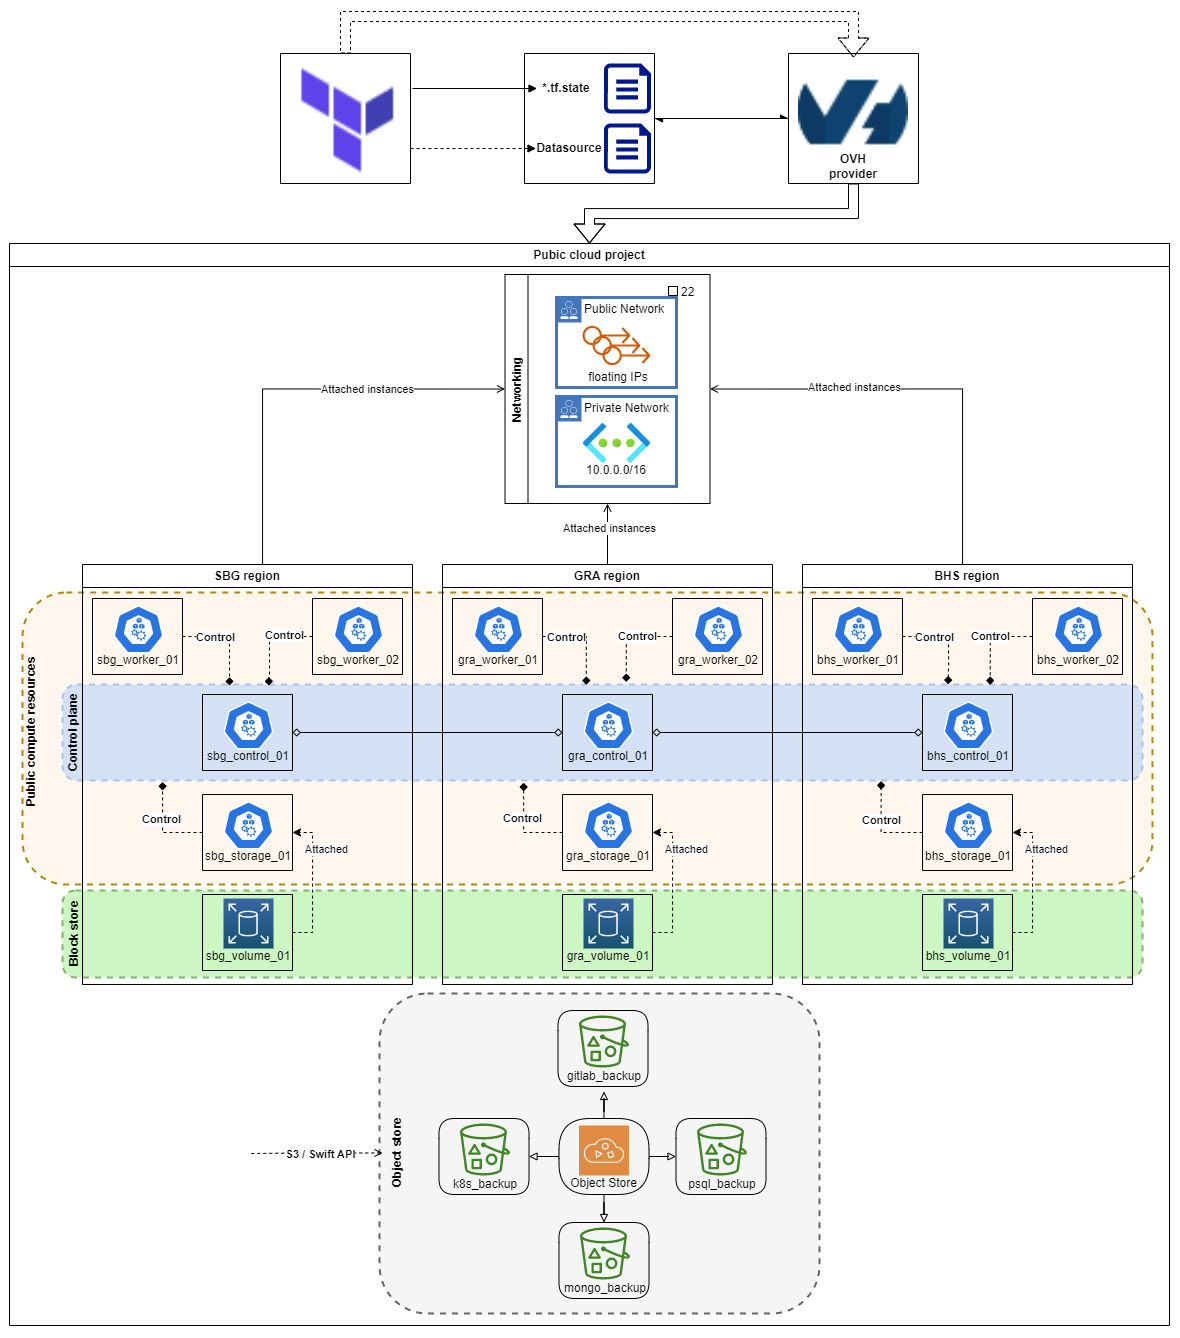
\includegraphics[width=1.0\textwidth,angle=00]{assets/f15.png}
\caption{Component diagram of provisioned resources}
\label{fig:fig15}
\end{figure}

The cluster resources were deployed to three regions. Namely, GRA, BHS, SBG. In each region, four instances were created. One of which will join the control plane, two will have the worker compute role and the last will have a second block device in raw format and will join the data storage backend. Various buckets from the object store will be provisioned and will serve as backup storage backends and high-speed data storage.  

\section*{Conclusion}

In conclusion, using Ansible and Terraform to provision and set up resources from OVH proved to be an efficient approach to setting up a PaaS environment on Kubernetes.  

The Terraform configuration provided a declarative way to describe the infrastructure and resources needed for the PaaS environment, while Ansible provided a reliable way to automate the configuration and deployment of the PaaS software stack on top of the infrastructure. 

Through this chapter, we leveraged OVH's cloud offerings to create infrastructure resources such as virtual machines, storage disks, and networks, and used Ansible to configure the instances and prepare them for the deployment of the PaaS environment. 

Overall, this approach offers a scalable and repeatable way to provision and deploy infrastructure and services on OVH.